\documentclass[
	aspectratio=169, % default is 43
	8pt, % font size, default is 11pt
	handout, % handout mode without animations, comment out to add animations
]{beamer}

\usepackage{../template/beamerthemeuulm} % use the inofficial uulm beamer theme
\setfaculty{infIngPsy} % set the color scheme for your faculty here [med/infIngPsy/math/nat]

% requires symbolic links
% git clone git@github.com:SoftVarE-Group/SlideTemplate.git C:\Users\...\SlideTemplate
% mklink /J template C:\Users\...\SlideTemplate
% git clone git@spgit.informatik.uni-ulm.de:thuem/slides.git C:\Users\...\ThomasSlides
% mklink /J thomasslides C:\Users\...\ThomasSlides
\graphicspath{{../template/pics/logos}{../template/pics/nature}{../template/pics/uulm}{../thomasslides/}{../pics/people/}{../pics/xkcd/}}

%\usepackage[ngerman]{babel} % use this line for slides in German
%\recordingtrue % special recording mode for use with a greenscreen, gives you space to show yourself in a layer in front of the slides, has no effect in the handout mode

\title{Software Product Lines} % short title is used for the slide footer but optional

% LINKED LITERATURE

\newcommand{\ludewiglichter}{\href{https://learning.oreilly.com/library/view/-/9781457184932/?ar}{Ludewig and Lichter}}
\newcommand{\seeconomics}{\href{https://rds-ulm.ibs-bw.de/link?kid=027381854}{SE Economics}}
\newcommand{\sommervillelink}[1]{\href{https://ulm.ibs-bw.de/aDISWeb/app?service=direct/0/Home/$DirectLink\&sp=SOPAC00\&sp=SAKSWB-IdNr1615420983}{#1}}
\newcommand{\sommerville}{\sommervillelink{Sommerville}}
\newcommand{\thehumbleprogrammer}{\href{https://dl.acm.org/doi/10.1145/1283920.1283927}{The Humble Programmer}}
\newcommand{\thepragmaticprogrammer}{\href{https://learning.oreilly.com/library/view/the-pragmatic-programmer/9780135956977/}{The Pragmatic Programmer}}

% TYPICAL COMMANDS FOR LECTURES

\renewcommand{\emph}[1]{{\color{blue}\textbf{#1}}}

\newcommand{\deutsch}[1]{{\color{blue}(#1)}}
\newcommand{\deutschertitel}[1]{{\tiny\deutsch{#1}}}

\newcommand{\mycite}[1]{``#1''}
\newcommand{\mytitlesource}[1]{{\tiny\normalfont\mbox{[#1]}}}
\newcommand{\mysource}[1]{\ifthenelse{\equal{#1}{}}{}{\phantom{.}~\hfill~\mytitlesource{#1}}}

\newcommand{\todo}[1]{{\color{red}\textbf{[#1]}}}
\newcommand{\fodo}[1]{\todo{\footnote{\todo{#1}}}}
\newcommand{\todots}{\todo{\ldots}}

% IMPORTED PACKAGES

%\usepackage{adjustbox} % used for partofpage
%\usepackage{tcolorbox} % used for mydefinition, mynote, myexample
\usepackage{multicol} % used temporarily for the lecture overview
\usepackage{mathtools} % required for absolute value in modeling lecture

% COMMANDS TO LAYOUT AND ANNIMATE SLIDES

\newcommand{\lessonslearned}[3]{
	\subsection{Summary}
	\begin{frame}{\insertsection -- \insertsubsection}
		\leftorright{
			\mydefinition{Lessons Learned}{
				\begin{itemize}
					#1
				\end{itemize}
			}
			\mynote{Further Reading}{
				\small % references take space, can be a little smaller
				\begin{itemize}
					#2
				\end{itemize}
			}
		}{
			\myexample{Practice}{
				#3
			}
		}
	\end{frame}
}

% TODO temporary hack to layout the slide overview in two colums
\renewcommand{\lectureoverview}{
%	\section*{Overview}
%	\subsection*{Overview}
	\begin{frame}{\insertsubtitle}
		\begin{multicols}{2}
			\tableofcontents
		\end{multicols}
	\end{frame}
}

\renewcommandx{\maketitle}[2][1=apr21-o25a,2=150]{
    {
	\usebackgroundtemplate{} % TODO temporary hack to enable missing pictures at title slide
	%\ifx {#1} \empty \else {\usebackgroundtemplate{\includegraphics[trim=0 0 0 #2,clip,width=\paperwidth]{#1}}} \fi     
	%\usebackgroundtemplate{\includegraphics[trim=0 0 0 #2,clip,width=\paperwidth]{#1}}
    \begin{frame}[plain]
        \vskip0pt plus 1filll
        \begin{beamercolorbox}[wd=\paperwidth,ht=4.5ex,dp=2ex,right]{titlebox}
            \LARGE\textbf{\inserttitle}\hspace*{20pt}
        \end{beamercolorbox}%
        \nointerlineskip%
        \begin{beamercolorbox}[wd=\paperwidth,ht=2.25ex,dp=1ex,right]{subtitlebox}
            \small 
            \ifx \insertsubtitle \empty \else \insertsubtitle\ $\vert$ \fi
            \insertauthor\
            \ifx \insertdate \empty \else $\vert$ \insertdate \fi
            \hspace*{20pt}
        \end{beamercolorbox}%
        \nointerlineskip%
        \begin{beamercolorbox}[wd=\paperwidth,ht=4.5ex,dp=2ex,left]{logobox}
            \centering
            \vspace{-1ex}
            \hspace{10pt}
            \includegraphics[height=4.5ex]{sp} % SPECIFY INSTITUTE LOGO HERE
            \hfill
            \includegraphics[height=4.5ex]{uulm}
            \hspace{10pt}
        \end{beamercolorbox}%
    \end{frame}
    }  
}

%
%\newcommand{\onlyleft}[1]{
%	\halfpage{#1}
%}
%
%\newcommand{\onlyright}[1]{
%	~\hfill
%	\halfpage{#1}
%}
%
%\newcommand{\leftorright}[2]{
%	\uncover<1>{\halfpage{#1}}
%	\hfill
%	\uncover<3->{\halfpage{#2}}
%}
%
%\newcommand{\rightorleft}[2]{
%	\uncover<3->{\halfpage{#1}}
%	\hfill
%	\uncover<1>{\halfpage{#2}}
%}
%
%\newcommand{\leftthenright}[2]{
%	\halfpage{#1}
%	\hfill\pause
%	\halfpage{#2}
%}
%
%\newcommand{\leftandright}[2]{
%	\halfpage{#1}
%	\hfill
%	\halfpage{#2}
%}
%
%\newcommand{\leftmiddleandright}[3]{
%	\thirdpage{#1}
%	\hfill
%	\thirdpage{#2}
%	\hfill
%	\thirdpage{#3}
%}
%
%\newcommand{\leftmiddleorright}[3]{
%	\uncover<1>{\thirdpage{#1}}
%	\hfill
%	\uncover<3>{\thirdpage{#2}}
%	\hfill
%	\uncover<5->{\thirdpage{#3}}
%}
%
%\newcommand{\halfpage}[1]{\partofpage{48}{#1}}
%
%\newcommand{\thirdpage}[1]{\partofpage{31}{#1}}
%
%\newcommand{\partofpage}[2]{
%	\adjustbox{valign=t}{\begin{minipage}{0.#1\textwidth}
%			\begin{flushleft}
%				#2
%			\end{flushleft}
%	\end{minipage}}
%}
%
%\newcommand{\mydefinition}[2]{
%	\begin{tcolorbox}[title=#1,colback=orange!10,colframe=orange!30,coltitle=black,fonttitle=\bfseries,left=1mm,right=1mm,top=1mm,bottom=1mm]
%		\begin{flushleft}
%			#2
%		\end{flushleft}
%	\end{tcolorbox}
%}
%
%\newcommand{\mydefinitiontight}[2]{
%	\begin{tcolorbox}[title=#1,colback=white,colframe=orange!30,coltitle=black,fonttitle=\bfseries,left=0mm,right=0mm,top=0mm,bottom=0mm]
%		\begin{flushleft}
%			#2
%		\end{flushleft}
%	\end{tcolorbox}
%}
%
%\newcommand{\mynote}[2]{
%	\begin{tcolorbox}[title=#1,colback=red!10,colframe=red!30,coltitle=black,fonttitle=\bfseries,left=1mm,right=1mm,top=1mm,bottom=1mm]
%		\begin{flushleft}
%			#2
%		\end{flushleft}
%	\end{tcolorbox}
%}
%
%\newcommand{\myexample}[2]{
%	\begin{tcolorbox}[title=#1,colback=blue!10,colframe=blue!30,coltitle=black,fonttitle=\bfseries,left=1mm,right=1mm,top=1mm,bottom=1mm]
%		\begin{flushleft}
%			#2
%		\end{flushleft}
%	\end{tcolorbox}
%}
%
%\newcommand{\myexampletight}[2]{
%	\begin{tcolorbox}[title=#1,colback=white,colframe=blue!30,coltitle=black,fonttitle=\bfseries,left=0mm,right=0mm,top=0mm,bottom=0mm]
%		\begin{flushleft}
%			#2
%		\end{flushleft}
%	\end{tcolorbox}
%}

\subtitle{11. Product-Line Testing}
\author{Thomas Thüm}

\begin{document}

\mode<handout>{\contentoverview}

\mode<beamer>{
	\ifdefined\thepicture
		\maketitle[\thepicture][\thepictureoffset]
	\else
		\maketitle[]
	\fi
}

% shared slide content

% introduced: 02a-configuration
% reused: 03a-intro
\newcommand{\frameImplementSPLs}{
	\begin{mycolumns}[widths={45},animation=none]
		\pic[width=\linewidth]{metaproduct2}
	\mynextcolumn
		\begin{note}{Key Issues}
			\begin{itemize}
			\item Systematic reuse of implementation artifacts
			\item Explicit handling of variability
			\end{itemize}
		\end{note}
		\uncover<2->{\begin{definition}{Variability\mysource{\fospl\mypage{48}}}
			\mycite{\emph{Variability} is the ability to derive different products from a common set of artifacts.}
		\end{definition}}
		~
		\uncover<3->{\begin{note}{Variability-Intensive System}
			Any software product line is a variability-intensive system. % TODO Timo: do we really need this term? where does this definition come from?
		\end{note}}
	\end{mycolumns}
}

% introduced: 02a-configuration
% reused: 02b-implementation, 03a-intro
\newcommand{\frameVariabilityAndBindingTimes}{
	\begin{mycolumns}[widths={55},animation=none]
		\begin{definition}{Binding Time \deutsch{Bindungszeitpunkt}\mysource{\fospl\mypage{48}}}
			\begin{itemize}
				\item Variability offers choices
				\item Derivation of a product requires to make decisions (aka. binding)
				\item Decisions may be bound at different binding times
			\end{itemize}
		\end{definition}
		~
		\uncover<2->{\begin{note}{When? By whom? How?}
			\lectureruntime\parta: \emph{when} and \emph{by whom}

			\lectureruntime\partb: \emph{how}
		\end{note}}
	\mynextcolumn
		\pic[width=\linewidth]{metaproduct2}
	\end{mycolumns}
}

% introduced: 03a-intro
% reused: 03a-intro
\newcommand{\frameRuntimeVariabilityProblems}{
	\begin{note}{Problems of Runtime Variability}
		{\bf Conditional Statements:}
		\begin{itemize}
			\item Code scattering, tangling, and replication
		\end{itemize}
		{\bf Design Patterns for Variability:}
		\begin{itemize}
			\item Trade-offs and potential negative side effects
			\item Constraints that may restrict their usage
		\end{itemize}
		{\bf In General:}
		\begin{itemize}
			\item Variable parts are always delivered
			\item Not well-suited for compile-time binding
		\end{itemize}
	\end{note}
}

% introduced: 03a-intro
% reused: 03a-intro
\newcommand{\frameSoftwareConfigurationManagement}{
	\begin{mycolumns}
		\begin{definition}{Software Configuration Management} % TODO source missing
			Policies, processes, and tools for managing evolving software systems:
			\begin{itemize}
				\item Version control
				\item System building
				\item Release management
				\item Change management
				\item Collaborative work
			\end{itemize}
		\end{definition}
	\mynextcolumn
		\begin{note}{No Software Configuration Management}
			\lecturecloneandown\parta: Ad-Hoc Clone-and-Own

			aka.\ unmanaged clone-and-own
		\end{note}
		\begin{note}{Version Control}
			\lecturecloneandown\partb: Clone-and-Own with Version Control

			instance of managed clone-and-own
		\end{note}
		\begin{note}{System Building}
			\lecturecloneandown\partc: Clone-and-Own with Build Systems

			instance of managed clone-and-own
		\end{note}
	\end{mycolumns}
}


\section{Product-Line Testing in Practice}

\begin{frame}{Recap: Software Quality}
	\rightorleft{
		\mydefinition{Quality \mysource{\ludewiglichter}}{Quality is the entirety of properties and characteristics of a product or process that indicate adequacy with respect to given requirements.}
		\mydefinition{Quality Assurance \mysource{\ludewiglichter}}{Quality assurance \deutsch{Qualitätssicherung} are all activities with the goal to improve the quality.}
	}{
		\vspace{-12mm}
		\href{https://commons.wikimedia.org/wiki/File:Andy_Hunt_programmer.jpg}{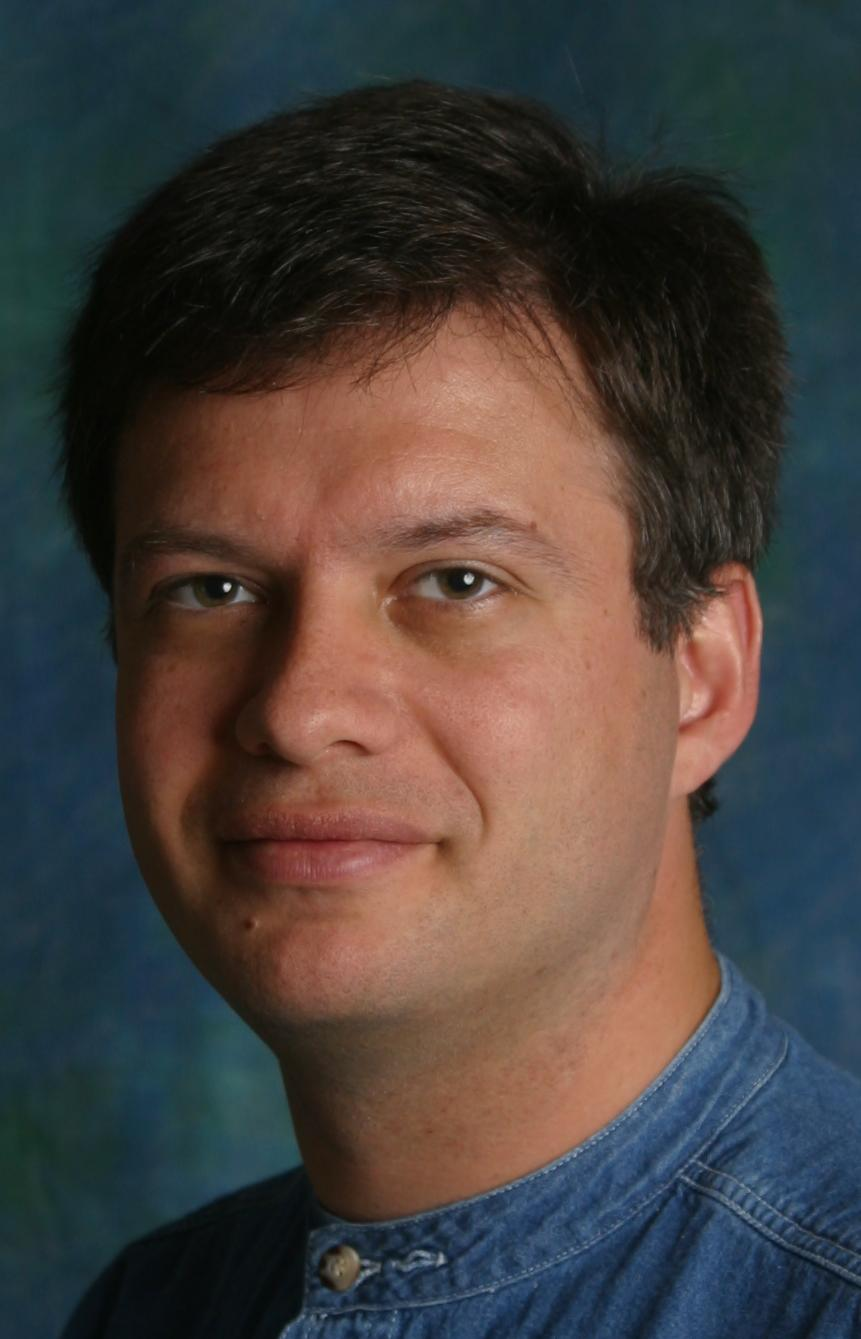
\includegraphics[width=\linewidth,trim=0 240 0 300,clip]{andy-hunt}}
		\vspace{-7mm}
		
		\mynote{Andy Hunt \mysource{\thepragmaticprogrammer}}{\mycite{No one in the brief history of computing has ever written a piece of perfect software. It's unlikely that you'll be the first.}}
		% co-authored The Pragmatic Programmer, known for the Agile Manifesto
	}
\end{frame}

\subsection{Recap: Quality Assurance}
\begin{frame}{Recap: Quality Assurance \mytitlesource{\ludewiglichter}}
	\vspace{-8mm}
	\hfill
	\todo{mindmap on quality assurance}
%	\begin{tikzpicture}
%		\path[small mindmap,
%		every node/.style={concept,font=\scriptsize},
%		emph/.style={font=\bfseries\scriptsize},
%		hide/.style={visible on=<1->},
%		concept color=uulmaccent!20,
%		level 1/.append style={level distance=25mm,sibling angle=360/6},
%		level 2/.append style={level distance=20mm,sibling angle=360/6},
%		level 3/.append style={level distance=20mm,sibling angle=360/8},
%		]
%		node {Quality Assurance \deutsch{Qualitätssicherung}}
%		[counterclockwise from=210]
%		child[visible on={<1->}] { node {constructive} 
%			[clockwise from=225]
%			child[concept color=blue!20] { node {Coding Guidelines} }
%		}
%		child[visible on={<2->}] { node {analytical} 
%			[counterclockwise from=240]
%			child[concept color=green!20,visible on={<3->}] { node {analysis}
%				[counterclockwise from=180]
%				child { node {Compilation} }
%				child { node {Code Reviews} }
%			}
%			child[concept color=red!20,visible on={<4->}] { node {execution}
%				[counterclockwise from=315]
%				child { node {White-Box Testing} }
%				child { node {Black-Box Testing} }
%			}
%		}
%		child[visible on={<5->}] { node {organizational} 
%			[clockwise from=-45]
%			child[concept color=orange!20] { node {Software Project Management} }
%		}
%		;
%	\end{tikzpicture}
\end{frame}

\begin{frame}{Recap: Software Testing}
	\leftorright{
		\vspace{7mm}
		\uncover<1-3>{\mydefinition{Software Testing \mysource{\sommerville}}{\mycite{Testing is intended to show that a program does what it is intended to do and to discover program defects before it is put into use.}}{}}
		\uncover<2-3>{\mydefinition{Validation Testing \mysource{\sommerville}}{\mycite{Demonstrate to the developer and the customer that the software meets its requirements.}}{}}
		\uncover<3-3>{\mydefinition{Defect Testing \mysource{\sommerville}}{\mycite{Find inputs or input sequences where the behavior of the software is incorrect, undesirable, or does not conform to its specification.}}{}}
	}{
		\vspace{-12mm}
		\uncover<4>{\mynote{V\&V \mysource{\seeconomics}}{\mycite{\emph{Validation}: Are we building the right product?\\\emph{Verification}: Are we building the product right?}}} 
		% TODO better visualization of V&V (see Inas slides). move to V model?
		\vspace{-2mm}
		\uncover<5>{\mynote{Stages of Testing \mysource{\sommerville}}{
			\begin{itemize}
				\setlength\itemsep{.1em}
				\item[1.] \mycite{\emph{Development testing}, where the system is tested during development to discover
				bugs and defects}
				\item[2.] \mycite{\emph{Release testing}, where a separate testing team tests a complete version of the
				system before it is released to users}
				\item[3.] \mycite{\emph{User testing}, where users or potential users of a system test the system in their
				own environment}
			\end{itemize}
		}}
		\vspace{-2mm}
		\uncover<6>{\mynote{}{\mycite{In \emph{manual testing}, a tester runs the program with some test data and
				compares the results to their expectations. [...] In \emph{automated testing}, the tests are encoded in a program that is run each time the system under development is to be tested.} \mysource{\sommerville}}}
	}
\end{frame}

\begin{frame}
	\leftorright{
		\href{https://commons.wikimedia.org/wiki/File:Edsger_Wybe_Dijkstra.jpg}{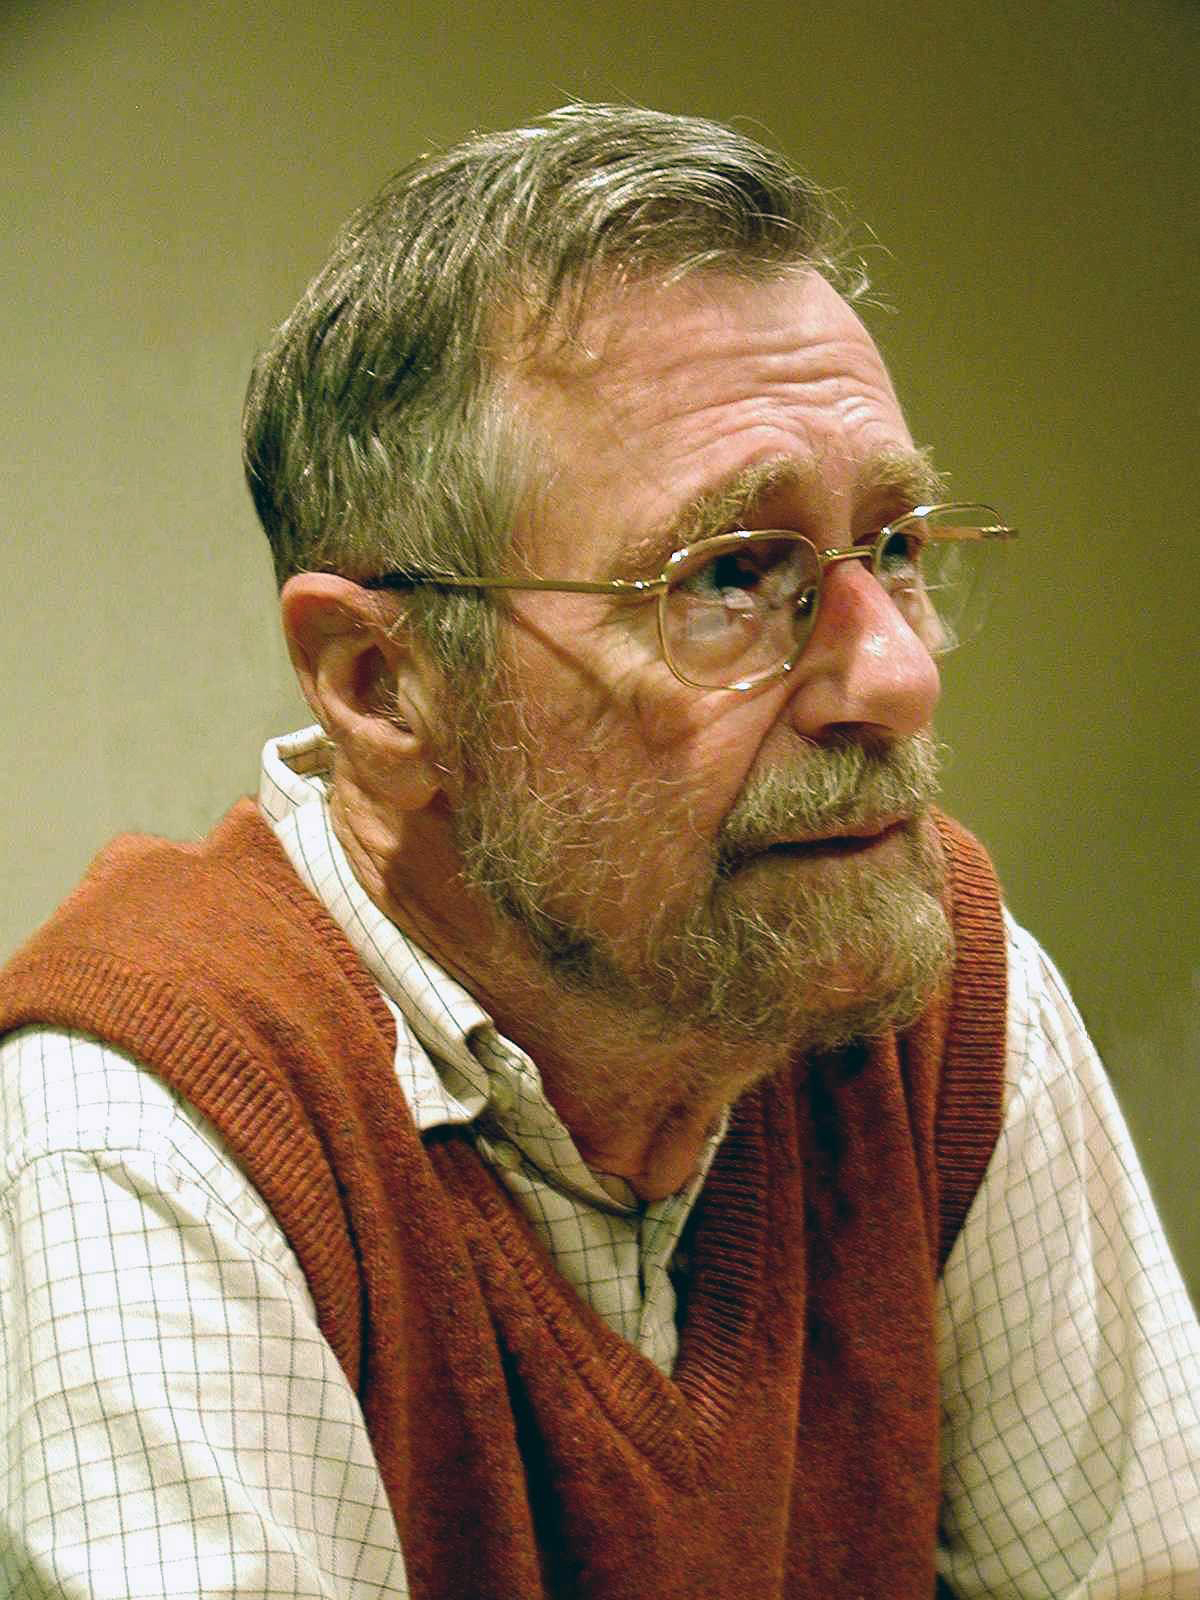
\includegraphics[width=\linewidth,trim=0 425 0 75,clip]{edsger-dijkstra}}
		\vspace{-7mm}
		
		\mynote{Edsger W. Dijkstra (1972) \mysource{\thehumbleprogrammer}}{\mycite{Program testing can be a very effective way to show the presence of bugs, but it is hopelessly inadequate for showing their absence.}}
		% 1930-2002, ACM Turing Award winner
	}{
		\todo{illustration for many configurations from previous slides}
	}
\end{frame}

\begin{frame}{Recap: Feature Model of the Linux Kernel}
	\vspace{28mm}~\hspace{-15mm}\href{https://dl.acm.org/doi/abs/10.1145/3382025.3414943}{\includegraphics[width=1.2\linewidth,page=1,trim=100 510 100 170,clip]{2020/2020-SPLC-Thuem}}
\end{frame}

% Dijkstra: we cannot test everything, and not all configurations
% complete test: all inputs, for all products/variants/configurations
% sampling technique (Stichprobenverfahren)
% recap: Testing All Configurations (remember numbers from intro? take 1ms per config)
% recap: Testing One Configuration (cp. allyesconfig, feature interactions may not be visible)

\subsection{Expert Knowledge in Sampling}

\subsection{Random Sampling}

\subsection{Excursus: Uniform Random Sampling}

\subsection{Testing the Linux Kernel}
% allyesconfig

%\subsection{Automation in Product Sampling} ???

%\subsection{Missing: Test-Case Selection/Generation}
% What to test for those configurations? Variable unit tests? Avoid redundant testing?

%\subsection{Slide Title 1}
\begin{frame}{~}
	\ldots
\end{frame}

\subsection{Slide Title 2}
\begin{frame}{-- Example Subtitle}
	\ldots
\end{frame}

\begin{frame}{-- Second Example Subtitle}
	\ldots
\end{frame}

\subsection{Slide Title 3}
%\begin{frame}{~}
%	\ldots
%\end{frame}



\lessonslearned{
	\item \ldots
}{
	\item \ldots
}{
	\ldots
}

\sectionend

\section{Combinatorial Interaction Testing}

\subsection{Test-Case Design in Single-System Engineering}
\begin{frame}{Recap: Test-Case Design \deutschertitel{Testfallentwurf}}
	\leftorright{
		\uncover<1>{\mydefinition{Systematic Test \mysource{\ludewiglichter}}{A systematic test is a test, in which
			\begin{itemize}
				\setlength\itemsep{.1em}
				\item[1.] the setup is defined,
				\item[2.] the inputs are chosen systematically,
				\item[3.] the results are documented and evaluated by criteria being defined prior to the test. 
			\end{itemize}
		}{}}
		\uncover<2>{\mydefinition{Test Case \mysource{\ludewiglichter}}{In a test, a number of test cases are executed, whereas each test case consists \emph{input values} for a single execution and \emph{expected outputs}. An \emph{exhaustive test} refers a test in which the test cases exercise all the possible inputs.}{}}
	}{
		\mynote{Goal \mysource{\ludewiglichter}}{Detect a large number of failures with a low number of test cases. A test case (execution) is \emph{positive}, if it detects a failure, and \emph{successful} if it detects an unknown failure.}
		\mydefinition{An ideal test case is \ldots \mysource{\ludewiglichter}}{
			\begin{itemize}
				\setlength\itemsep{.1em}
				\item representative: represents a large number of feasible test cases
				\item failure sensitive: has a high probability to detect a failure
				\item non-redundant: does not check what other test cases already check
			\end{itemize}
		}{}
	}
\end{frame}

\begin{frame}{Recap: Black-Box Testing \mytitlesource{\ludewiglichter}}
	\leftandright{
		\mynote{Motivation}{
			\begin{itemize}
				\setlength\itemsep{.1em}
				\item source code not always available (e.g., outsourced components, obfuscated code)
				\item specific test cases derived from logical ones using arbitrary values
				\item specification not incorporated so far (only for expected results)
				\item invalid inputs not tested
				\item errors are not equally distributed
			\end{itemize}
		}
		\vspace{-1mm}
		\mydefinition{Black-Box Testing \deutsch{Funktionstest}}{
			\begin{itemize}
				\setlength\itemsep{.1em}
				\item test-case design based on specification
				\item source code and its inner structure is ignored (assumed as a black-box)
			\end{itemize}
		}{}
	}{
	}
\end{frame}

\subsection{Pairwise Interaction Testing}

\subsection{A Greedy Algorithm}

\subsection{Meta-Heuristic Search}

\subsection{T-Wise Interaction Testing}

\subsection{Effectiveness of Combinatorial Interaction Testing}

\subsection{Efficiency of Combinatorial Interaction Testing}
% testing efficiency and sampling efficiency

%\subsection{Slide Title 1}
\begin{frame}{~}
	\ldots
\end{frame}

\subsection{Slide Title 2}
\begin{frame}{-- Example Subtitle}
	\ldots
\end{frame}

\begin{frame}{-- Second Example Subtitle}
	\ldots
\end{frame}

\subsection{Slide Title 3}
%\begin{frame}{~}
%	\ldots
%\end{frame}



\lessonslearned{
	\item \ldots
}{
	\item \ldots
}{
	\ldots
}

\sectionend

\section{Solution-Space Sampling}

\subsection{Coverage in Single-System Engineering}
\begin{frame}{Recap: Coverage in White-Box Testing \mytitlesource{\ludewiglichter}}
	\vspace{-7mm}
	\leftorright{
		\mydefinition{White-Box Testing \deutsch{Strukturtest}}{
			\begin{itemize}
				\setlength\itemsep{.1em}
				\item inner structure of test object is used
				\item idea: coverage of structural elements
				\item code translated into control flow graph
				\item specific test case (concrete inputs)\\derived from logical test case (conditions)\\derived from path in control flow graph
			\end{itemize}
		}{}
	}{
		\mydefinition{Coverage Criteria \deutsch{Überdeckungskriterien}}{
			\begin{itemize}
				\setlength\itemsep{.1em}
				\item[1.] statement coverage \deutsch{Anweisungsüberdeck.}: all statements are executed for at least one test case
				\uncover<3->{\item[2.] branching coverage \deutsch{Zweigüberdeckung}: statement coverage and for each branching statement all branches have been exercised} % TODO not so easy to define as percentage
				\uncover<4->{\item[3.] term coverage \deutsch{Termüberdeckung}: branching coverage and terms ($n$) used in a branching statement are combined exhaustively ($2^n$)\hfill(simplified)}
				% TODO discuss path coverage?
			\end{itemize}
		}{}
	}
\end{frame}

\subsection{Coverage of Ifdef Blocks}

\subsection{Presence-Condition Coverage}

%\subsection{Encoding Solution Space in Feature Models}

\subsection{Overview on Coverage Criteria}

\subsection{Overview on Input for Sampling Algorithms}
% include test cases as input

%\subsection{Slide Title 1}
\begin{frame}{~}
	\ldots
\end{frame}

\subsection{Slide Title 2}
\begin{frame}{-- Example Subtitle}
	\ldots
\end{frame}

\begin{frame}{-- Second Example Subtitle}
	\ldots
\end{frame}

\subsection{Slide Title 3}
%\begin{frame}{~}
%	\ldots
%\end{frame}



\lessonslearned{
	\item \ldots
}{
	\item \ldots
}{
	\ldots
}

\mode<beamer>{
	\begin{frame}{\inserttitle}
		\lectureseriesoverview
	\end{frame}

	\contentoverview
}


%\begin{frame}{Example}
%	\includegraphics[width=\linewidth,page=3,trim=0 40 0 40,clip]{2D Analysis/2019-10-17 SPP1593 2Danalysis.pdf}
%\end{frame}

\end{document}
